\documentclass{article}
\usepackage[margin=1in]{geometry}
\usepackage[utf8]{inputenc}
\usepackage{amsmath}
\usepackage{tikz}
\usepackage{pgfplots}
\pgfplotsset{compat=1.18}
\usepackage{color}
\usepackage{amsfonts}
\usepackage{amssymb}
\usepackage{graphicx}

\title{Homework 3}
\author{Giacomo Cappelletto}
\date{\today}

\begin{document}

\maketitle

\section*{Problem 1 - Section A}

\subsection*{System 1}

\subsubsection*{A}
\begin{figure}[h!]
	\centering
	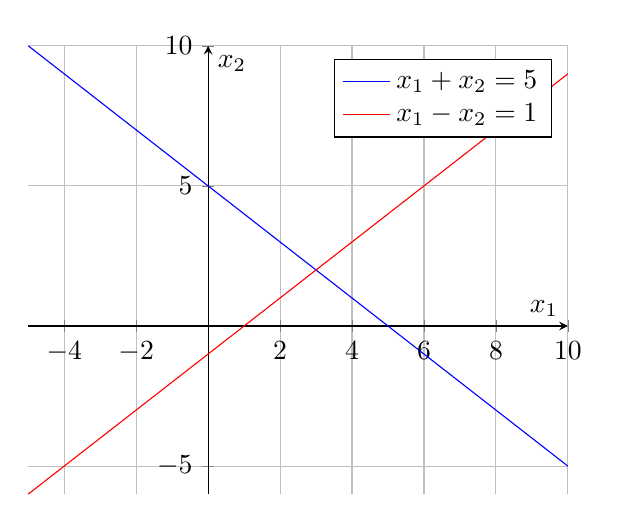
\begin{tikzpicture}
		\begin{axis}[
				axis lines = middle,
				xlabel = $x_1$,
				ylabel = $x_2$,
				grid = both,
				legend pos = north east
			]
			% Plot of x + y = 5
			\addplot[
				domain=-5:10,
				samples=20,
				color=blue
			]
			{5 - x};
			\addlegendentry{$x_1 + x_2 = 5$}

			% Plot of x - y = 1
			\addplot[
				domain=-5:10,
				samples=20,
				color=red
			]
			{x - 1};
			\addlegendentry{$x_1 - x_2 = 1$}


		\end{axis}
	\end{tikzpicture}
	\caption{Plot of $x_1 + x_2 = 5$ and $x_1 - x_2 = 1$}
	\label{fig:plot1}
\end{figure}

\subsubsection*{B}

A unique solution since there is one intersection point between the lines.

\subsubsection*{C}

\[
	\begin{bmatrix}
		1 & 1  \\
		1 & -1
	\end{bmatrix}
	\cdot
	\begin{bmatrix}
		x_1 \\
		x_2
	\end{bmatrix}
	=
	\begin{bmatrix}
		5 \\
		1
	\end{bmatrix}
\]

\subsubsection*{D}

\[
	\begin{bmatrix}
		1 & 1  & 5 \\
		1 & -1 & 1
	\end{bmatrix}
\]

\subsubsection*{E}

\[
	\begin{bmatrix}
		1 & 1  & 5 \\
		1 & -1 & 1
	\end{bmatrix}
	\xrightarrow{R_2 = R_2 - R_1}
	\begin{bmatrix}
		1 & 1  & 5  \\
		0 & -2 & -4
	\end{bmatrix}
\]

\subsubsection*{F}

\[
	\begin{bmatrix}
		1 & 1  & 5  \\
		0 & -2 & -4
	\end{bmatrix}
	\xrightarrow{R_2 = -\frac{1}{2}R_2}
	\begin{bmatrix}
		1 & 1 & 5 \\
		0 & 1 & 2
	\end{bmatrix}
	\xrightarrow{R_1 = R_1 - R_2}
	\begin{bmatrix}
		1 & 0 & 3 \\
		0 & 1 & 2
	\end{bmatrix}
\]

Therefore, given this RREF, it follows that

\[
	\begin{bmatrix}
		x_1 \\
		x_2
	\end{bmatrix}
	=
	\begin{bmatrix}
		3 \\
		2
	\end{bmatrix}
\]

\subsection*{System 2}

\subsubsection*{A}

\begin{figure}[h!]
	\centering
	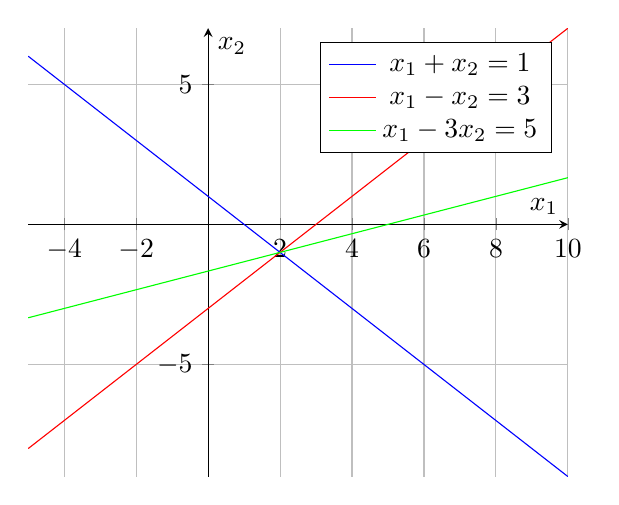
\begin{tikzpicture}
		\begin{axis}[
				axis lines = middle,
				xlabel = $x_1$,
				ylabel = $x_2$,
				grid = both,
				legend pos = north east
			]
			% Plot of x + y = 5
			\addplot[
				domain=-5:10,
				samples=20,
				color=blue
			]
			{1 - x};
			\addlegendentry{$x_1 + x_2 = 1$}

			% Plot of x - y = 1
			\addplot[
				domain=-5:10,
				samples=20,
				color=red
			]
			{x - 3};
			\addlegendentry{$x_1 - x_2 = 3$}

			% Plot of x - y = 1
			\addplot[
				domain=-5:10,
				samples=20,
				color=green
			]
			{(x/3) - (5/3)};
			\addlegendentry{$x_1 - 3x_2 = 5$}


		\end{axis}
	\end{tikzpicture}
	\caption{Plot of $x_1 + x_2 = 1$, $x_1 - x_2 = 3$, and $x_1 - 3x_2 = 5$}
	\label{fig:plot2}
\end{figure}

\subsubsection*{B}

The SLE will have one solution since all lines intersect at the same point.

\subsubsection*{C}

\[
	\begin{bmatrix}
		1 & 1  \\
		1 & -1 \\
		1 & -3
	\end{bmatrix}
	\cdot
	\begin{bmatrix}
		x_1 \\
		x_2
	\end{bmatrix}
	=
	\begin{bmatrix}
		1 \\
		3 \\
		5
	\end{bmatrix}
\]

\subsubsection*{D}

\[
	\begin{bmatrix}
		1 & 1  & 1 \\
		1 & -1 & 3 \\
		1 & -3 & 5
	\end{bmatrix}
\]

\subsubsection*{E}

\[
	\begin{bmatrix}
		1 & 1  & 1 \\
		1 & -1 & 3 \\
		1 & -3 & 5
	\end{bmatrix}
	\xrightarrow{R_2 = R_2 - R_1, R_3 = R_3 - R_1}
	\begin{bmatrix}
		1 & 1  & 1 \\
		0 & -2 & 2 \\
		0 & -4 & 4
	\end{bmatrix}
	\xrightarrow{R_3 = R_3 - 2R_2}
	\begin{bmatrix}
		1 & 1  & 1 \\
		0 & -2 & 2 \\
		0 & 0  & 0
	\end{bmatrix}
\]

\[
	\begin{bmatrix}
		1 & 1  & 1 \\
		0 & -2 & 2 \\
		0 & 0  & 0
	\end{bmatrix}
	\xrightarrow{R_2 = -\frac{1}{2}R_2}
	\begin{bmatrix}
		1 & 1 & 1  \\
		0 & 1 & -1 \\
		0 & 0 & 0
	\end{bmatrix}
	\xrightarrow{R_1 = R_1 - R_2}
	\begin{bmatrix}
		1 & 0 & 2  \\
		0 & 1 & -1 \\
		0 & 0 & 0
	\end{bmatrix}
\]
Therefore, given this RREF, it follows that

\[
	\begin{bmatrix}
		x_1 \\
		x_2
	\end{bmatrix}
	=
	\begin{bmatrix}
		2 \\
		-1
	\end{bmatrix}
\]

\subsection*{System 3}

\subsubsection*{A}

\begin{figure}[h!]
	\centering
	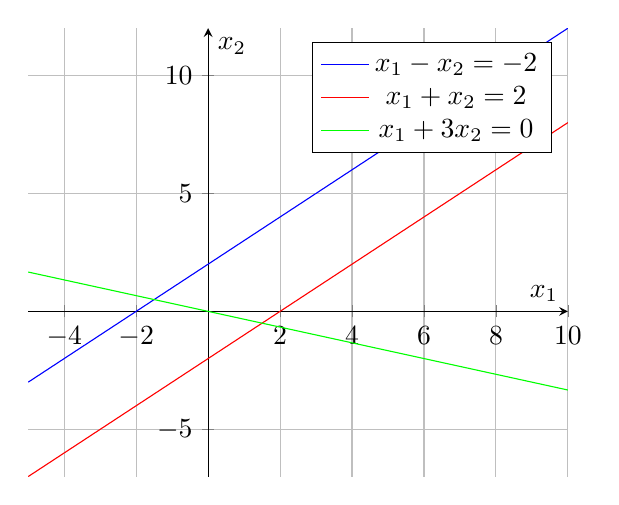
\begin{tikzpicture}
		\begin{axis}[
				axis lines = middle,
				xlabel = $x_1$,
				ylabel = $x_2$,
				grid = both,
				legend pos = north east
			]
			\addplot[
				domain=-5:10,
				samples=20,
				color=blue
			]
			{x+2};
			\addlegendentry{$x_1 - x_2 = -2$}

			\addplot[
				domain=-5:10,
				samples=20,
				color=red
			]
			{x - 2};
			\addlegendentry{$x_1 + x_2 = 2$}

			\addplot[
				domain=-5:10,
				samples=20,
				color=green
			]
			{-x/3};
			\addlegendentry{$x_1 + 3x_2 = 0$}

		\end{axis}
	\end{tikzpicture}
	\caption{Plot of $x_1 - x_2 = -2$, $x_1 + x_2 = 2$, and $x_1 + 3x_2 = 0$}
	\label{fig:plot3}
\end{figure}

\subsubsection*{B}

No solution to SLE since the lines do not all have common intersection point.

\subsubsection*{C}

\[
	\begin{bmatrix}
		1 & 1 \\
		1 & 1 \\
		1 & 3
	\end{bmatrix}
	\cdot
	\begin{bmatrix}
		x_1 \\
		x_2
	\end{bmatrix}
	=
	\begin{bmatrix}
		-2 \\
		2  \\
		0
	\end{bmatrix}
\]

\subsubsection*{D}

\[
	\begin{bmatrix}
		1 & -1 & -2 \\
		1 & 1  & 2  \\
		1 & 3  & 0
	\end{bmatrix}
\]

\subsubsection*{E}

\[
	\begin{bmatrix}
		1 & -1 & -2 \\
		1 & 1  & 2  \\
		1 & 3  & 0
	\end{bmatrix}
	\xrightarrow{R_2 = R_2 - R_1 ,R_3 = R_3 - R_1}
	\begin{bmatrix}
		1 & -1 & 2 \\
		0 & 2  & 4 \\
		0 & 4  & 2
	\end{bmatrix}
	\xrightarrow{R_3 = R_3 - 2R_2}
	\begin{bmatrix}
		1 & -1 & 2  \\
		0 & 2  & 4  \\
		0 & 0  & -6
	\end{bmatrix}
\]

\subsubsection*{F}

The last column of the REF effectively shows that $x_1 \cdot 0 = -6$, which is sufficient to determine that the SLE is not consistent.

\section*{Problem 1 - Section B}

\subsection*{System 4}

\begin{figure}[h!]
	\centering
	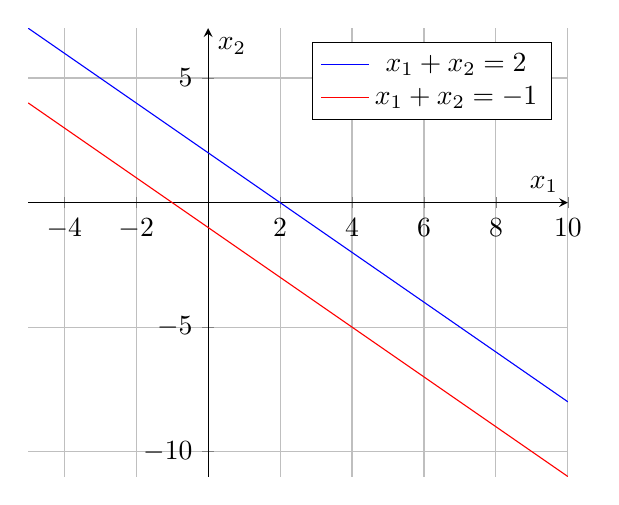
\begin{tikzpicture}
		\begin{axis}[
				axis lines = middle,
				xlabel = $x_1$,
				ylabel = $x_2$,
				grid = both,
				legend pos = north east
			]
			% Plot of x + y = 5
			\addplot[
				domain=-5:10,
				samples=20,
				color=blue
			]
			{2 - x};
			\addlegendentry{$x_1 + x_2 = 2$}

			% Plot of x - y = 1
			\addplot[
				domain=-5:10,
				samples=20,
				color=red
			]
			{-x - 1};
			\addlegendentry{$x_1 + x_2 = -1$}


		\end{axis}
	\end{tikzpicture}
	\caption{Plot of $x_1 + x_2 = 2$ and $x_1 + x_2 = -1$}
	\label{fig:plot4}
\end{figure}

\subsubsection*{B}

The SLE will have no solutions since the lines are parallel and therefore will never intersect.

\subsubsection*{C}

\[
	\begin{bmatrix}
		1 & 1 & 2  \\
		1 & 1 & -2
	\end{bmatrix}
	\xrightarrow{R_2 = R_2 - R_1}
	\begin{bmatrix}
		1 & 1 & 2 \\
		0 & 0 & 4
	\end{bmatrix}
	\xrightarrow{R_2 = -\frac{1}{4}R_2}
	\begin{bmatrix}
		1 & 1 & 2 \\
		0 & 0 & 1
	\end{bmatrix}
	\xrightarrow{R_1 = R_1 - 2R_2}
	\begin{bmatrix}
		1 & 1 & 0 \\
		0 & 0 & 1
	\end{bmatrix}
\]

\subsubsection*{D}

\begin{verbatim}
    A = [1,1;1,1];
    disp(rref(A))
    \end{verbatim}

\color{lightgray}
\begin{verbatim}
        1     1
        0     0
\end{verbatim}
\color{black}

\subsubsection*{E}

\begin{verbatim}
    A = [1,1,2;1,1,-2];
    disp(rref(A))
\end{verbatim}

\color{lightgray}
\begin{verbatim}
         1     1     0
         0     0     1
    
\end{verbatim}
\color{black}


\subsubsection*{F}

\[
	\begin{bmatrix}
		\tikz[baseline=(char.base)] \node[draw,circle,inner sep=2pt] (char) {1}; & 1 & 0                                                                         \\
		0                                                                        & 0 & \tikz[baseline=(char.base)] \node[draw,circle,inner sep=2pt] (char)  {1};
	\end{bmatrix}
\]

Column 1: Pivot
Column 2: Free variable
Column 3: Pivot

\subsubsection*{G}

Since there is a pivot in the last column, from which is follows that $x_2 \cdot 0 = 1$, the SLE is in fact not consistent.

\subsection*{System 5}

\begin{figure}[h!]
	\centering
	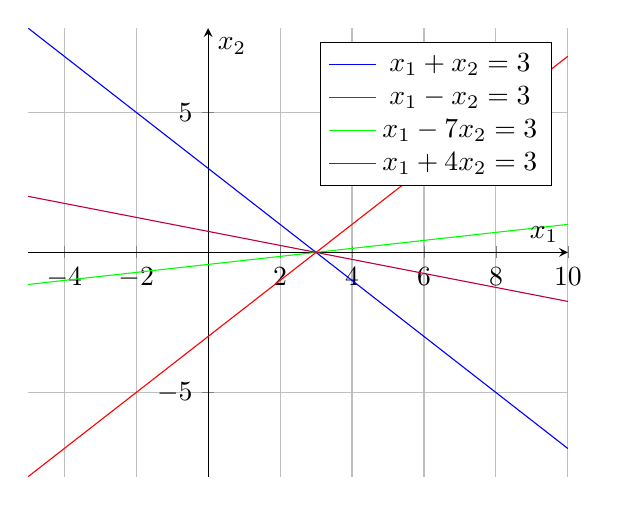
\begin{tikzpicture}
		\begin{axis}[
				axis lines = middle,
				xlabel = $x_1$,
				ylabel = $x_2$,
				grid = both,
				legend pos = north east
			]
			\addplot[
				domain=-5:10,
				samples=20,
				color=blue
			]
			{3-x};
			\addlegendentry{$x_1 + x_2 = 3$}
			\addplot[
				domain=-5:10,
				samples=20,
				color=red
			]
			{x-3};
			\addlegendentry{$x_1 - x_2 = 3$}
			\addplot[
				domain=-5:10,
				samples=20,
				color=green
			]
			{(x/7)-(3/7)};
			\addlegendentry{$x_1 - 7x_2 = 3$}
			\addplot[
				domain=-5:10,
				samples=20,
				color=purple
			]
			{(3/4)-(x/4)};
			\addlegendentry{$x_1 + 4x_2 = 3$}


		\end{axis}
	\end{tikzpicture}
	\caption{Plot of $x_1 + x_2 = 3$, $x_1 - x_2 = 3$, $x_1 - 7x_2 = 3$, and $x_1 + 4x_2 = 3$}
	\label{fig:plot5}
\end{figure}

\subsubsection*{B}

Unique solution since there exists a common intersection point of the lines.

\subsubsection*{C}

\[
	\begin{bmatrix}
		1 & 1  & 3 \\
		1 & -1 & 3 \\
		1 & -7 & 3 \\
		1 & 4  & 3
	\end{bmatrix}
	\xrightarrow{R_2 = R_2 - R_1, R_3 = R_3 - R_1, R_4 = R_4 - R_1}
	\begin{bmatrix}
		1 & 1  & 3 \\
		0 & -2 & 0 \\
		0 & -8 & 0 \\
		0 & 3  & 0
	\end{bmatrix}
	\xrightarrow{R_4=2R_4}
	\begin{bmatrix}
		1 & 1  & 3 \\
		0 & -2 & 0 \\
		0 & -8 & 0 \\
		0 & 6  & 0
	\end{bmatrix}
\]
\[
	\xrightarrow{R_4=R_4+3R_3, R_3=R_3-4R_2}
	\begin{bmatrix}
		1 & 1  & 3 \\
		0 & -2 & 0 \\
		0 & 0  & 0 \\
		0 & 0  & 0
	\end{bmatrix}
	\xrightarrow{R_2=-frac{1}{2}R_2}
	\begin{bmatrix}
		1 & 1 & 3 \\
		0 & 1 & 0 \\
		0 & 0 & 0 \\
		0 & 0 & 0
	\end{bmatrix}
	\xrightarrow{R_1=R_1-R_2}
	\begin{bmatrix}
		1 & 0 & 3 \\
		0 & 1 & 0 \\
		0 & 0 & 0 \\
		0 & 0 & 0
	\end{bmatrix}
\]
\subsubsection*{D}


\begin{verbatim}
    A = [1,1;1,-1;1,3;1,4];
    disp(rref(A))
\end{verbatim}

\color{lightgray}
\begin{verbatim}
         1     0
         0     1
         0     0
         0     0
\end{verbatim}
\color{black}


\subsubsection*{E}

\begin{verbatim}
    A = [1,1,3;1,-1,3;1,-7,3;1,4,3];
    disp(rref(A))
\end{verbatim}

\color{lightgray}
\begin{verbatim}
         1     0     3
         0     1     0
         0     0     0
         0     0     0
    
\end{verbatim}
\color{black}

\subsubsection*{F}

\[
	\begin{bmatrix}
		\tikz[baseline=(char.base)] \node[draw,circle,inner sep=2pt] (char) {1}; & 0                                                                        & 3 \\
		0                                                                        & \tikz[baseline=(char.base)] \node[draw,circle,inner sep=2pt] (char) {1}; & 0 \\
		0                                                                        & 0                                                                        & 0 \\
		0                                                                        & 0                                                                        & 0
	\end{bmatrix}
\]

Column 1: Pivot
Column 2: Pivot

\subsubsection*{G}

Yes, the SLE is indeed consistent and unique as predicted. By expanding the augmented matrix back to two equations we are left with $x_1 = 3, x_2 = 0$, which is indeed the same point shown in Fig.\ref{fig:plot5}.

\subsection*{System 6}

\subsubsection*{A}

-

\subsubsection*{B}

Since there are 3 equations in 5 unknowns, if the system is consistent it must have infinitely many solutions (with two free variables).

\subsubsection*{C}

\[
	\begin{bmatrix}
		1  & 1 & 1  & 1  & 1 & 4 \\
		-1 & 1 & -1 & 1  & 1 & 2 \\
		2  & 2 & 0  & -1 & 5 & 4
	\end{bmatrix}
	\xrightarrow{R_2 = R_2 + R_1,\quad R_3 = R_3 - 2R_1}
	\begin{bmatrix}
		1 & 1 & 1  & 1  & 1 & 4  \\
		0 & 2 & 0  & 2  & 2 & 6  \\
		0 & 0 & -2 & -3 & 3 & -4
	\end{bmatrix}
\]
\[
	\xrightarrow{R_2 = \frac{1}{2}R_2,\quad R_3 = -\frac{1}{2}R_3}
	\begin{bmatrix}
		1 & 1 & 1 & 1           & 1            & 4 \\
		0 & 1 & 0 & 1           & 1            & 3 \\
		0 & 0 & 1 & \frac{3}{2} & -\frac{3}{2} & 2
	\end{bmatrix}
\]
\[
	\xrightarrow{R_1 = R_1 - R_2}
	\begin{bmatrix}
		1 & 0 & 1 & 0           & 0            & 1 \\
		0 & 1 & 0 & 1           & 1            & 3 \\
		0 & 0 & 1 & \frac{3}{2} & -\frac{3}{2} & 2
	\end{bmatrix}
\]
\[
	\xrightarrow{R_1 = R_1 - R_3}
	\begin{bmatrix}
		1 & 0 & 0 & -\frac{3}{2} & \frac{3}{2}  & -1 \\
		0 & 1 & 0 & 1            & 1            & 3  \\
		0 & 0 & 1 & \frac{3}{2}  & -\frac{3}{2} & 2
	\end{bmatrix}
\]

\subsubsection*{D}

\begin{verbatim}
    A = [1,1,1,1,1;-1,1,-1,1,1;2,2,0,-1,5];
    disp(rref(A))
    \end{verbatim}
\color{lightgray}
\begin{verbatim}
             1.0000    0         0   -1.5000    1.5000
             0    1.0000         0    1.0000    1.0000    
             0         0    1.0000    1.5000   -1.5000    
\end{verbatim}
\color{black}

\subsubsection*{E}

\begin{verbatim}
    A = [1,1,1,1,1,4;-1,1,-1,1,1,2;2,2,0,-1,5,4];
    disp(rref(A))
    \end{verbatim}
\color{lightgray}
\begin{verbatim}
             1.0000    0         0   -1.5000    1.5000   -1.0000
             0    1.0000         0    1.0000    1.0000    3.0000
             0         0    1.0000    1.5000   -1.5000    2.0000
\end{verbatim}
\color{black}

\subsubsection*{F}

Column 1: Pivot
Column 2: Pivot
Column 3: Pivot
Column 4: Free Variable
Column 5: Free Variable

\subsubsection*{G}

Given the RREF, and asssuming $x_4 = t_4, x_5 = t_5$, it can be deduced that

\[
	\begin{aligned}
		x_1 & = -1 + \frac{3}{2}t_4 - \frac{3}{2}t_5, \\
		x_2 & = 3 - t_4 - t_5,                        \\
		x_3 & = 2 - \frac{3}{2}t_4 + \frac{3}{2}t_5.
	\end{aligned}
\]

Therefore, demonstrating the aforementioned proposition system is consistent and not unique, but has infinitely many solutions.

\section*{Problem 2}

\subsection{A}
\subsubsection*{$A\vec{v}=\vec{b}$}
\[
	\begin{bmatrix}
		1  & 1  & 1 \\
		1  & -3 & 0 \\
		-1 & 2  & 6
	\end{bmatrix}
	\cdot
	\begin{bmatrix}
		x_1 \\
		x_2 \\
		x_3
	\end{bmatrix}
	=
	\begin{bmatrix}
		2 \\ 1 \\ 5
	\end{bmatrix}
\]
\subsubsection*{$[A | \vec{v} ]$}

\[
	\begin{bmatrix}
		1  & 1  & 1 & 2 \\
		1  & -3 & 0 & 1 \\
		-1 & 2  & 6 & 5
	\end{bmatrix}
\]

\subsection*{B}

\[
	\begin{bmatrix}
		1  & 1  & 1 & 2 \\
		1  & -3 & 0 & 1 \\
		-1 & 2  & 6 & 5
	\end{bmatrix}
	\xrightarrow{R_2 = R_2 - R_1,\; R_3 = R_3 + R_1}
	\begin{bmatrix}
		1 & 1  & 1  & 2  \\
		0 & -4 & -1 & -1 \\
		0 & 3  & 7  & 7
	\end{bmatrix}
	\xrightarrow{R_3 = R_3 + \frac{3}{4}R_2}
	\begin{bmatrix}
		1 & 1  & 1            & 2            \\
		0 & -4 & -1           & -1           \\
		0 & 0  & \frac{25}{4} & \frac{25}{4}
	\end{bmatrix}
\]

\subsection*{C}
\[
	\begin{bmatrix}
		\tikz[baseline=(char.base)] \node[draw,circle,inner sep=2pt] (char){1}; & 1                                                                        & 1                                                                                    & 2            \\
		0                                                                       & \tikz[baseline=(char.base)] \node[draw,circle,inner sep=2pt] (char){-4}; & -1                                                                                   & -1           \\
		0                                                                       & 0                                                                        & \tikz[baseline=(char.base)] \node[draw,circle,inner sep=2pt] (char){$\frac{25}{4}$}; & \frac{25}{4}
	\end{bmatrix}
\]

\subsection*{D}

\[
	\begin{bmatrix}
		1 & 1  & 1            & 2            \\
		0 & -4 & -1           & -1           \\
		0 & 0  & \frac{25}{4} & \frac{25}{4}
	\end{bmatrix}
	\xrightarrow{R_2 = -\frac{1}{4}R_2,\; R_3 = \frac{4}{25}R_3}
	\begin{bmatrix}
		1 & 1 & 1           & 2           \\
		0 & 1 & \frac{1}{4} & \frac{1}{4} \\
		0 & 0 & 1           & 1
	\end{bmatrix}
	\xrightarrow{R_2 = R_2 - \frac{1}{4}R_3}
	\begin{bmatrix}
		1 & 1 & 1 & 2 \\
		0 & 1 & 0 & 0 \\
		0 & 0 & 1 & 1
	\end{bmatrix}
\]
\[
	\xrightarrow{R_1 = R_1 - R_3}
	\begin{bmatrix}
		1 & 1 & 0 & 1 \\
		0 & 1 & 0 & 0 \\
		0 & 0 & 1 & 1
	\end{bmatrix}
	\xrightarrow{R_1 = R_1 - R_2}
	\begin{bmatrix}
		1 & 0 & 0 & 1 \\
		0 & 1 & 0 & 0 \\
		0 & 0 & 1 & 1
	\end{bmatrix}
\]

\subsection*{E}

\begin{verbatim}
    A = [1,1,1; 1,-3,0; -1,2,6];
    b= [2;1;5]
    x = A \ b
\end{verbatim}

\color{lightgray}
\begin{verbatim}
    b =
    
         2
         1
         5
    
    
    x =
    
         1
         0
         1
    
\end{verbatim}
\color{black}

\subsection*{G}


\begin{verbatim}
    % \\\\\\\\\\\\\\\\\\\\\\\\\\\\\\\\\\\\\\\\\\\\\\\\\\\\\\\\\\\\\\\\\\\
    %     Problem 2:  Plotting 3 intersecting planes
    %
    % \\\\\\\\\\\\\\\\\\\\\\\\\\\\\\\\\\\\\\\\\\\\\\\\\\\\\\\\\\\\\\\\\
    
    
    % -- Suppose we have an Ax = b equation, where A = (3 x 3), and it
    %    representes these 3 equations:
    
    
    %   Plane #1:        x1  +  x2  +  x3  = 2
    %   Plane #2:        x1  -  x2  + 2x3  = 3
    %   Plane #3:       -x1  + 2x2  + 4x3  = 3
    
    % -- Define matrix A
    
    A = [ 1  1  1 ;       % -- row vector r1
          1 -3  0 ;       % -- row vector r2
         -1  2  6 ]       % -- row vector r3
    
    %    a1 a2 a3         % -- Column vectors a1, a2, a3
    
    
    % -- Define target vector b
    b = [ 2 1 5 ]'
    
    
    % -- We can solve for x by using the \  command:
    
    disp('The solution to our Ax = b problem is');
    x = A\b
    
    
    % \\\\\\\\\\\\\\\\\\\\\\\\\\\\\\\\\\\\\\\\\\\\\\\\\\\\\\\\\\
    %
    %   Task 1:    Drawing the 3 planes of interest
    %
    %   We will learn how to do this later when we talk about nullspace
    %   solutions.  For now, just trust the code here =)
    %
    %
    %   Sub-tasks:
    % ---------------------------------------------------
    %
    % -- 1.  Extract the row vectors r1, r2, r3 from matrix A
    %
    % -- 2.  Then, we will find the nullspace vectors to the equation
    %                 r' * xn1  = 0
    %                 r' * xn2  = 0
    %
    % -- 3.  Then, will draw the plane spanned by the 2 nullspace vectors
    %        xn1 and xn2
    %
    % \\\\\\\\\\\\\\\\\\\\\\\\\\\\\\\\\\\\\\\\\\\\\\\\\\\\\\\\\\
    
    
    % -- Define my own color pallet
    
    my_colormap = [ 1  0.6  0     ;   % --- orange
                    0   1   0     ;   % --  green
                    0   0   1 ];      % --  blue
    
    
    % -- Create a new figure
    figure;
    
    
    % -- Forcing the new figure to have a certain size on your screen
    %    and at a certain position
    set(gcf, 'Position',  [100, 100, 700, 600])
    
    
    % --  Iterate over each row vector r1, r2, r3
    
    for count = 1:1:3
    
        r1 = A(count,:);    % -- Extract the row vector (r1, r2, r3)
    
        % -- First, we will auto-calculate the:
        %    a)  Particular solution:  my_xp
        %    b)  Nullspace vector #1:  my_xn1
        %    c)  Nullspace vector #2:  my_xn2
    
    
        xp  = [ b(count)       0  0 ]' / r1(1);
        xn1 = [ -r1(2)/r1(1)   1  0 ]' ;
        xn2 = [ -r1(3)/r1(1)   0  1 ]' ;
    
    
        % -- Then, we will plot the plane spanned by my_xn1
        %                                            my_xn2
        %    with the centroid of the plane at:      xp
    
        % -- Now, we will use the "patch" command to draw a 2D plane that
        %    represents the span{xn1, xn2}
        %
        %    These are the coordinates for the 4 corners of the plane
        %
        %
        %    Point Q                                                Point M
        %
        %   2*(-xn1+xn2)       ----------------------------- 2*(xn1 + xn2)
        %                     |            |              |
        %                     |            |              |
        %                      <--------   xp --------------->
        %                     |            |              |
        %    Point P          |            |              |         Point N
        %                     |            |              |
        %  2*(-xn1-xn2)      -----------------------------2*(xn1 - xn22)
        %
    
    
        % -- We can change the size + scale of our plane by using this
        %    magnification factor
    
        my_scale = 2;
    
    
        % -- Compute the cooridnates for the 4 corners.  The data structure
        %    here looks like this:
        %
        %                 Points: [   M       N        P          Q   ]  + xp
        % --------------------------------------------------------------------
        my_corners = my_scale .* [ xn1+xn2  xn1-xn2 -xn1-xn2  -xn1+xn2 ] + xp;
    
        % -- Plot the plane using the patch command  (# of vertices = 4)
        %
        %
        % Syntax:  my_plothandle = patch( 'XData', [ xcoords ],
        %                                 'YData', [ ycoords ],
        %                                 'ZData', [ zcoords ] );
    
        my_plane_plothandle(count) = patch('XData', my_corners(1,:), 'YData', my_corners(2,:), 'ZData', my_corners(3,:));
        set(my_plane_plothandle(count), 'FaceColor', my_colormap(count,:), 'FaceAlpha', 0.2)
    
        hold on;
    
    end
    
    
    % \\\\\\\\\\\\\\\\\\\\\\\\\\\\\\\\\\\\\\\\\\\\\\\\\\\\\\\\\\\
    %
    %   Task #2:  Plot the solution vector x  (the answer) as a
    %             big black dot
    %
    %   ** You will have to change the "my_x" vector to have it
    %      plotted correctly !!
    %
    % \\\\\\\\\\\\\\\\\\\\\\\\\\\\\\\\\\\\\\\\\\\\\\\\\\\\\\\\\\
    
    % -- Define solution vector
    x_solution = [ 1  0  1 ]';   %  <---  you need to change this !!
    
    
    % -- Plot it as a black dot using the "plot3" command:
    
    x_solution_plothandle = plot3( x_solution(1), x_solution(2), x_solution(3), '.');
    set(x_solution_plothandle, 'Color', 'black', 'Markersize', 30);
    
    
    % -- cosmetics for the plot
    xmin = -5;
    xmax = 5;
    ymin = -5;
    ymax = 5;
    zmin = -5;
    zmax = 5;
    
    % -- Using "axis square" will ensure equally-spaced grid lines
    %    across all 3 axes x, y, z !!
    
    grid on;
    axis([xmin xmax ymin ymax zmin zmax]);
    axis square;
    
    xlabel('x1-axis');
    ylabel('x2-axis');
    zlabel('x3-axis');
    title('Problem 1:  3 intersecting planes (unique solution)');
    
    
    % \\\\\\\\\\\\\\\\\\\\\\\\\\\\\\\\\\\\\\\\\\\\\\\\\\\\\\\\\\
    % -- Create legend strings
    %
    % -- We will extract the row vector numbers from matrix A using the
    %    num2str( ) command !!
    %
    % \\\\\\\\\\\\\\\\\\\\\\\\\\\\\\\\\\\\\\\\\\\\\\\\\\\\\\\\\\
    
    my_legend_strings = { };  % -- Initialize string matrix
    
    for count = 1:1:3
    
        % -- Creat the legend strings for each plan
        %    Note:  "32"  =  space bar (in ASCII code)
    
        my_legend_strings{count} = strcat( 'Plane #', num2str(count), ':', 32, num2str(A(count,1)), 'x_1 + ', num2str(A(count,2)), 'x_2 + ', num2str(A(count,3)), 'x_3 = ', 32, num2str(b(count)));
    
    end
    
    % -- Then, add the 4th legend (the x = solution black dot)
     my_legend_strings{count+1}  = strcat( 'x_{solution} = [ ', 32, num2str(x_solution'), 32, ']^T'  );
    
    % -- Plot the legend itself
    %
    %                                 plothandles         , string matrix
    %                      -------------------------------------------------
    my_legend_plothandle = legend( [ my_plane_plothandle   x_solution_plothandle  ], my_legend_strings);
    set(my_legend_plothandle, 'FontName', 'Arial', 'Fontsize', 9);
    
    % -- Release the hold on the plot
    hold off;
    
    
    % -- 3D camera position (so that you can view the 3D planes at a
    %    convenient perpsective)
    
    campos([66.5824   49.0335   25.7390]);
    \end{verbatim}

\color{lightgray} \begin{verbatim}
    A =
    
         1     1     1
         1    -3     0
        -1     2     6
    
    
    b =
    
         2
         1
         5
    
    The solution to our Ax = b problem is
    
    x =
    
         1
         0
         1
    
    \end{verbatim}
\color{black}

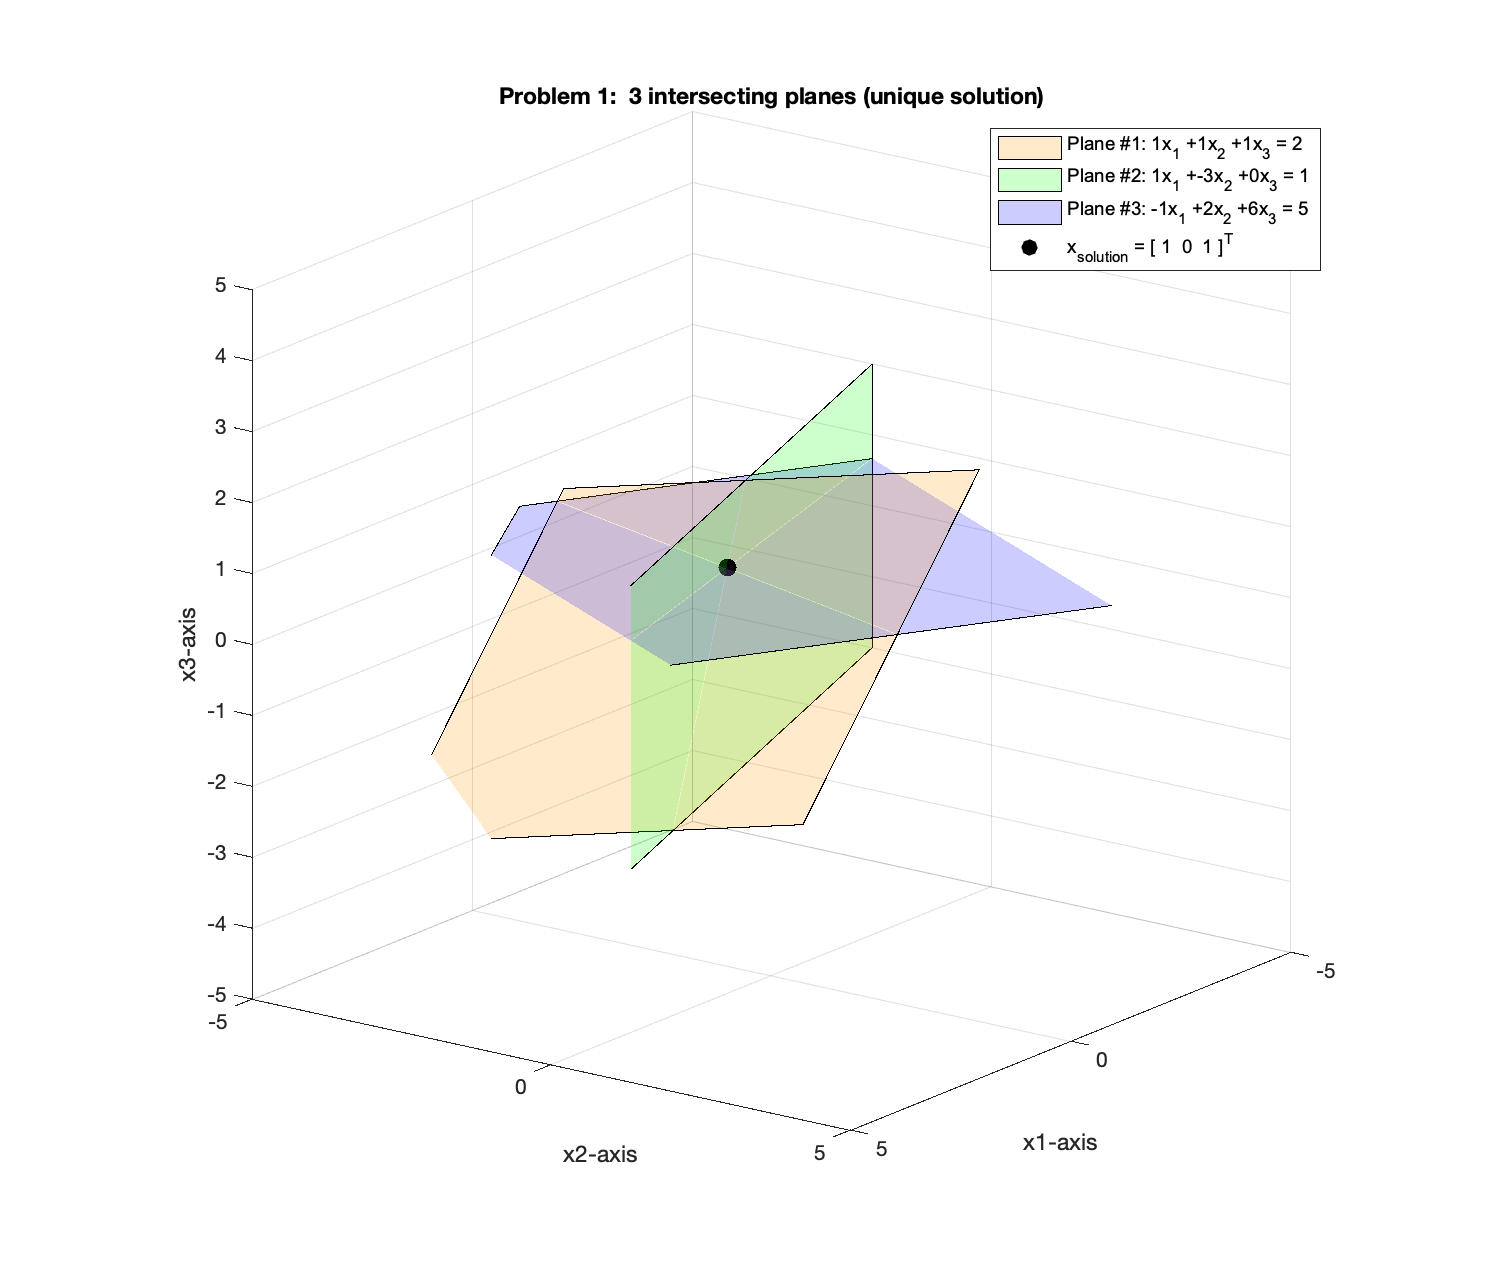
\includegraphics [width=5in]{Problem2_2Dplanes_unique_01.eps}


\section*{Problem 3}

\subsection*{A}
\subsubsection*{$A\vec{x}=\vec{b}$}
\[
	\begin{bmatrix}
		2 & -1 & 1  \\
		1 & 1  & -2
	\end{bmatrix}
	\cdot
	\begin{bmatrix}
		x_1 \\
		x_2 \\
		x_3
	\end{bmatrix}
	=
	\begin{bmatrix}
		2 \\ 0
	\end{bmatrix}
\]
\subsubsection*{$[A | \vec{b} ]$}

\[
	\begin{bmatrix}
		2 & -1 & 1  & 2 \\
		1 & 1  & -2 & 0
	\end{bmatrix}
\]

\subsection*{B}

\[
	\begin{bmatrix}
		2 & -1 & 1  & 2 \\
		1 & 1  & -2 & 0
	\end{bmatrix}
	\xrightarrow{R_2 = R_2 - 2R_1}
	\begin{bmatrix}
		2  & -1 & 1  & 2  \\
		-3 & 3  & -4 & -4
	\end{bmatrix}
	\xrightarrow{R_1 = \frac{1}{2}R_1,\; R_2 = -\frac{1}{3}R_2}
	\begin{bmatrix}
		1 & -\frac{1}{2} & \frac{1}{2} & 1           \\
		1 & -1           & \frac{4}{3} & \frac{4}{3}
	\end{bmatrix}
\]
\[
	\xrightarrow{R_2 = R_2 - R_1}
	\begin{bmatrix}
		1 & -\frac{1}{2} & \frac{1}{2} & 1           \\
		0 & -\frac{1}{2} & \frac{5}{6} & \frac{1}{3}
	\end{bmatrix}
	\xrightarrow{R_2 = -2R_2}
	\begin{bmatrix}
		1 & -\frac{1}{2} & \frac{1}{2}  & 1            \\
		0 & 1            & -\frac{5}{3} & -\frac{2}{3}
	\end{bmatrix}
	\xrightarrow{R_1 = R_1 + \frac{1}{2}R_2}
	\begin{bmatrix}
		1 & 0 & -\frac{1}{3} & \frac{2}{3}  \\
		0 & 1 & -\frac{5}{3} & -\frac{2}{3}
	\end{bmatrix}
\]

\subsection*{C}

\begin{verbatim}
    A = [2,-1,1,2; 1,1,-2,0];
    disp(rref(A))
    \end{verbatim}
\color{lightgray}
\begin{verbatim}
             1.0000  0        -0.3333    0.6667
             0       1.0000   -1.6667   -0.6667
    \end{verbatim}
\color{black}

\subsection*{D}

\[
	\begin{bmatrix}
		\tikz[baseline=(char.base)] \node[draw,circle,inner sep=2pt] (char){1}; & 0                                                                       & -\frac{1}{3} & \frac{2}{3}  \\
		0                                                                       & \tikz[baseline=(char.base)] \node[draw,circle,inner sep=2pt] (char){1}; & -\frac{5}{3} & -\frac{2}{3}
	\end{bmatrix}
\]

Column 1: Pivot
Column 2: Pivot
Column 3: Free Variable

\subsection*{E}

Given the RREF matrix, setting the free variable $x_3 = t_3$, we can then formulate the solutio to the SLE As

\[
	\begin{aligned}
		x_1 - \frac{1}{3}t_3 = \frac{2}{3} \\
		x_2 - \frac{5}{3}t_3 = -\frac{2}{3}
		x_3 = t_3
	\end{aligned}
\]

Which solved for $x_1, x_2$ gives

\[
	\begin{bmatrix}
		x_1 \\
		x_2 \\
		x_3
	\end{bmatrix}
	=
	\begin{bmatrix}
		\frac{2}{3}  \\
		-\frac{2}{3} \\
		0
	\end{bmatrix}
	+
	t_3
	\begin{bmatrix}
		\frac{1}{3} \\
		\frac{5}{3} \\
		1
	\end{bmatrix}
\]

Which is the parametric form of a line, which is indeed the intersection between two planes, and therefore has an infinite number of points lying on it.

\subsection*{F}

Since the intersection between the planes is a line (they are not parallel or identical) the we can parametrise this line and iterate over it with a scalar parameter ($t_3$) to get an infinite number of points which satisfies the SLE.

\subsection*{G}

\[
	\begin{bmatrix}
		2 & -1 & 1  \\
		1 & 1  & -2
	\end{bmatrix}
	\begin{bmatrix}
		\frac{2}{3}  \\
		-\frac{2}{3} \\
		0
	\end{bmatrix}
	=
	\begin{bmatrix}
		2\cdot\frac{2}{3} + (-1)\cdot\left(-\frac{2}{3}\right) + 1\cdot 0 \\
		1\cdot\frac{2}{3} + 1\cdot\left(-\frac{2}{3}\right) + (-2)\cdot 0
	\end{bmatrix}
\]
\[
	=\begin{bmatrix}
		\frac{4}{3} + \frac{2}{3} \\
		\frac{2}{3} - \frac{2}{3}
	\end{bmatrix}
	=\begin{bmatrix}
		\frac{6}{3} \\
		0
	\end{bmatrix}
	=\begin{bmatrix}
		2 \\
		0
	\end{bmatrix}.
\]

\section*{Problem 4}

\subsection*{A}
\subsubsection*{$A\vec{x}=\vec{b}$}
\[
	\begin{bmatrix}
		1 & 0 & 10 \\
		2 & 0 & 2  \\
		2 & 0 & -2
	\end{bmatrix}
	\cdot
	\begin{bmatrix}
		x_1 \\
		x_2 \\
		x_3
	\end{bmatrix}
	=
	\begin{bmatrix}
		4 \\-2\\2
	\end{bmatrix}
\]

\subsubsection*{$[A | \vec{b} ]$}

\[
	\begin{bmatrix}
		1 & 0 & 10 & 4 \\2&0&2&-2\\2&0&-2&2
	\end{bmatrix}
\]

\subsection*{B}

\[
	\begin{bmatrix}
		1 & 0 & 10 & 4  \\
		2 & 0 & 2  & -2 \\
		2 & 0 & -2 & 2  \\
	\end{bmatrix}
	\xrightarrow{R_2 = R_2 - 2R_1, R_3 = R_3 - 2R_1}
	\begin{bmatrix}
		1 & 0 & 10  & 4   \\
		0 & 0 & -18 & -10 \\
		0 & 0 & -22 & -6
	\end{bmatrix}
	\xrightarrow{R_3 = R_3 - \frac{11}{9}R_2}
	\begin{bmatrix}
		1 & 0 & 10  & 4            \\
		0 & 0 & -18 & -10          \\
		0 & 0 & 0   & \frac{56}{9}
	\end{bmatrix}
\]

\subsection*{C}

By expanding the last row of the REF matrix, we are presented with $0 \cdot x_3 = \frac{56}{9}$, which is not a valid equation and therefore proves that the SLE is not consistent as for any value $k \in \mathbb{R}$ for $x_3$ would yield $0 = \frac{56}{9}$ which is false.

\subsection*{D}


\begin{verbatim}
	A = [1,0,10,4; 2,0,2,-2;2,0,-2,2];
	disp(rref(A))
\end{verbatim}

\color{lightgray} 
\begin{verbatim}
		1     0     0     0
		0     0     1     0
		0     0     0     1
\end{verbatim} 
\color{black}

\subsection*{E}

Once again, this RREF matrix is not consistent, as the last row, expanded, gives $0 \cdot x_3 = 1$, which deems the SLE as not consistent as for any value $k \in \mathbb{R}$ for $x_3$ would yield $0 = 1$ which is false.

\end{document}



